\hypertarget{sensor-fusion}{%
\section{\texorpdfstring{\texttt{Sensor\ Fusion}}{Sensor Fusion}}\label{sensor-fusion}}

\hypertarget{simple-example-of-sensor-fusion}{%
\subsection{Simple Example of Sensor
Fusion}\label{simple-example-of-sensor-fusion}}

Consider a system with \(n\) sensors each making a single measurement:

\[z_i, \quad i=1, \dots, n\]

of some unknown quantity \(x\). The measurements really are described by

\[z_i = x + v_i,  \quad i=1, \dots, n .\]

We seek an optimal estimate of \(x\) based on a linear combination of
these measurements:

\[\hat{x} = \sum_{i=1}^n k_i z_i .\]

How should we proceed? It is a matter of writing down an expression for
the error in the estimate and minimizing the error.

We will assume that the noise \(v_i\) is zero mean white noise (normally
distributed) and independent. Thus we have that

\[E(v_i) =0, \quad \mbox{and} \quad E(v_i v_j) = 0, \quad i\neq j,\]

where \(E(x)\) is the expected value of \(x\). We want the estimate to
be unbiased which means that \(E(\hat{x}-x) = 0\). We define optimality
as minimizing the mean square error:

\[E[(\hat{x}-x)^2].\]

\textbf{Lemma 1} \(E[\hat{x}-x]=0\) implies \(\sum_{i=1}^n k_i = 1\)

An unbiased estimate means that \(E(\hat{x}-x) = 0\),

\begin{quote}
\[E[\hat{x}-x] = E\left[\sum_{i=1}^n k_i z_i - x\right] = E\left[\sum_{i=1}^n k_i (x+v_i) - x\right]\]

\[= E\left[\sum_{i=1}^n k_i x - x + \sum_{i=1}^n k_i v_i\right]
= \sum_{i=1}^n k_i E[x] - E[x]  + \sum_{i=1}^n k_i E[v_i] = 0\]
\end{quote}

since \(E(v_i)=0\) and \(E(x)=x\) we have that

\begin{quote}
\[\sum_{i=1}^n k_i = 1 .\]
\end{quote}

\textbf{Lemma 2} \(E[(\hat{x}-x)^2] =  \sum_{i=1}^n k_i^2\sigma_i^2\)

where \(\sigma_i\) are the standard deviations for \(v_i\),
\(E((v-E(v))^2)=\sigma^2\).

\[E[(\hat{x}-x)^2] =  E\left[\left(\sum_{i=1}^n k_i z_i - x\right)^2\right]
=  E\left[\left(\sum_{i=1}^n k_i (x+v_i) - x\right)^2\right]\]

\[= E\left[\left(\sum_{i=1}^n k_i x - x + \sum_{i=1}^n k_i v_i \right)^2\right]=
E\left[\left(\sum_{i=1}^n k_i v_i \right)^2\right]\]

\[=E\left[\sum_{i=1}^n \sum_{j=1}^n k_ik_j v_iv_j \right]
= \sum_{i=1}^n \sum_{j=1}^n k_ik_j E[v_iv_j] = \sum_{i=1}^n k_i^2\sigma_i^2 .\]

\hypertarget{optimal-estimate}{%
\subsubsection{\texorpdfstring{\texttt{Optimal\ Estimate}}{Optimal Estimate}}\label{optimal-estimate}}

The main goal is to minimize the mean square error subject to the
constraint of having the unbiased estimate:

\begin{itemize}
\tightlist
\item
  Minimize \(\sum_{i=1}^n k_i^2\sigma_i^2\) (minimize mean square
  error),
\item
  Subject to \(\sum_{i=1}^n k_i = 1\) (unbiased estimate).
\end{itemize}

We proceed using Lagrange Multipliers which will allow us to optimize a
constrained function. Expressing as the Lagrangian

\[L = \sum_{i=1}^n k_i^2\sigma_i^2 - \lambda \left( \sum_{i=1}^n k_i - 1\right)\]

we must solve

\[\nabla_k L =0 \quad \text{with} \quad \sum_{i=1}^n k_i = 1 .\]

Thus

\[\nabla L =
\left[ 2k_1\sigma_1^2 - \lambda , 2k_2\sigma_2^2 - \lambda, \dots, 2k_n\sigma_n^2 - \lambda\right]=\vec{0}\]

\[\sum_{i=1}^n k_i = 1\]

Solve for \(k_i\) in each gradient equation and sum

\[\sum_{i=1}^n k_i =  \sum_{i=1}^n \frac{\lambda}{2\sigma_i^2} = 1\]

So, we have that

\[\lambda =  \left(\displaystyle\sum_{i=1}^n \displaystyle \frac{1}{2\sigma_i^2}\right)^{-1}\]

This provides \(k_i\)

\[k_i = \frac{1}{\sigma_i^2} \left(\displaystyle\sum_{i=1}^n \displaystyle \frac{1}{\sigma_i^2}\right)^{-1}\]

and we obtain the estimate

\[\hat{x} = \displaystyle \frac{\displaystyle \sum_{i=1}^n \frac{z_i}{\sigma_i^2}}
{\displaystyle \sum_{i=1}^n \frac{1}{\sigma_i^2}}.\]

From \texttt{Lem:varianceformula} we can also gain an estimate of the
variance for the estimate, \(\hat{x}\) above:

\[\sigma^2 =  \sum_{i=1}^n k_i^2\sigma_i^2 =  \sum_{i=1}^n\left( \frac{1}{\sigma_i^2} \left(\displaystyle\sum_{i=1}^n \displaystyle \frac{1}{\sigma_i^2}\right)^{-1}\right)^2 \sigma_i^2\]

\[=  \left(\displaystyle\sum_{i=1}^n \displaystyle \frac{1}{\sigma_i^2}\right)^{-2} \sum_{i=1}^n\left( \frac{1}{\sigma_i^2} \right) =  \left(\displaystyle\sum_{i=1}^n \displaystyle \frac{1}{\sigma_i^2}\right)^{-1}\]

\hypertarget{simple-example-using-uniform-variance}{%
\subsection{Simple example using uniform
variance}\label{simple-example-using-uniform-variance}}

If the variances are the same, \(\sigma_i = \sigma\), then

\[\sum_{i=1}^n \frac{1}{\sigma_i^2} = \frac{1}{\sigma^2} \sum_{i=1}^n 1 = \frac{n}{\sigma^2}\]

and so

\[\hat{x} = \displaystyle \frac{\displaystyle \frac{1}{\sigma^2} \sum_{i=1}^n z_i}
{\displaystyle \frac{n}{\sigma^2}} = \displaystyle \frac{1}{n} \sum_{i=1}^n z_i\]

which is the average.

\hypertarget{dataexamplediffvar}{%
\subsection{Example with different variances}\label{dataexamplediffvar}}

Say you measure something three different ways and you want to merge
these measurements into a single estimate. How does one specifically go
about it. Assume that the three devices do return normally distributed
measurements. But what is the actual distribution? Keep in mind for
normal distributions, we only need to track the mean and standard
deviation and those are complete descriptors for the distribution.

Recall that the mean and the standard deviation are

\[\mu = \frac{1}{n}\sum_{i=1}^n x_i, \quad\quad\sigma = \sqrt{\frac{1}{n-1} \sum_{i=1}^n (x_i - \mu)^2}\]

Assume that you sample three sensors with 20 measurements each for some
experiment. The data you gain is

\begin{verbatim}
2.28333   1.87365    2.12419
2.26493   1.77675    1.80968
2.33626   1.85706    2.00608
2.13676   1.83520    2.12145
... (middle removed to fit)
2.14289   1.86792    1.86616
2.21151   1.88855    2.20027
2.17112   1.95257    1.77513
2.19798   1.82083    2.25617
Means:
2.20548   1.85962    2.04204
Standard Deviations:
0.08698   0.04282    0.17674
\end{verbatim}

The normal curves for the three sensors are

\[P_i(x|\mu, \sigma) = \displaystyle\frac{1}{\sigma_i\sqrt{2\pi}}\, e^{\displaystyle-\frac{(x-\mu_i)^2}{2\sigma_i^2}}\]

and are given in \texttt{normalcurves}.

\begin{quote}
The normal curves for the three sensors. Sensor A is shown in red,
sensor B in green and sensor C in blue.
\end{quote}

Assume the experimental setup was such that the true measurement was
2.0. The difference between the true measurement and the sensor average
constitutes the systematic error. It is a constant bias term which can
be removed. You need to compute the difference between the true value
and the dataset average. This provides the amount you need to shift your
measurement value:

\begin{verbatim}
Shift data
x shift (add) =  -0.205476607108
y shift (add) =  0.140376647675
z shift (add) =  -0.0420388951565






The shifted curves for the three sensors. Sensor A is shown in red,
sensor B in green and sensor C in blue.
\end{verbatim}

Once you have the standard deviations, we can perform a single
measurement using the three sensor and then merge the three into a
single estimate of the state. Assume you get the following measurements
for sensors A, B and C respectively: 2.22685 1.90326 2.17253. Then the
corrected measurements for sensors A, B and C are \(z_1 = 2.02137\),
\(z_2 =  2.04363\), \(z_3 =  2.13049\).

Using the weighted sum derived above, we can fuse the measurements based
on standard deviations.

\[\hat{x} = \displaystyle \frac{\displaystyle \sum_{i=1}^n \frac{z_i}{\sigma_i^2}}{\displaystyle
\sum_{i=1}^n \frac{1}{\sigma_i^2}} =
\displaystyle \frac{\displaystyle  \frac{ 2.02137}{0.08698^2} + \frac{2.04363}{0.04282^2}    + \frac{2.13049}{0.17674^2}  }{\displaystyle
 \frac{ 1}{0.08698^2} + \frac{1}{0.04282^2}    + \frac{1}{0.17674^2}  } = 2.0434 .\]

The variance for this measurement is given by \(\sigma^2 =\)

\[\left(\displaystyle\sum_{i=1}^n \displaystyle \frac{1}{\sigma_i^2}\right)^{-1}
 = \left( {\displaystyle
 \frac{ 1}{0.08698^2} + \frac{1}{0.04282^2}    + \frac{1}{0.17674^2}  } \right)^{-1}
 \approx 0.0375404^2\]

Note that the standard deviation is lower than all three of the
estimates, meaning the fused measurement is more accurate than any of
the measurements alone.

The code to implement the data fusion is given below. We assume we
already have three Numpy arrays (the sensor data arrays) filled with the
20 sensor test readings.

\begin{Shaded}
\begin{Highlighting}[]
\KeywordTok{using}\NormalTok{ Statistics}
\KeywordTok{using}\NormalTok{ Formatting}

\NormalTok{a\_shift }\OperatorTok{=} \FloatTok{2.0} \OperatorTok{{-}}\NormalTok{ mean(sensor\_a\_data)}
\NormalTok{b\_shift }\OperatorTok{=} \FloatTok{2.0} \OperatorTok{{-}}\NormalTok{ mean(sensor\_b\_data)}
\NormalTok{c\_shift }\OperatorTok{=} \FloatTok{2.0} \OperatorTok{{-}}\NormalTok{ mean(sensor\_c\_data)}

\NormalTok{a\_std }\OperatorTok{=}\NormalTok{ std(sensor\_a\_data)}
\NormalTok{b\_std }\OperatorTok{=}\NormalTok{ std(sensor\_b\_data)}
\NormalTok{c\_std }\OperatorTok{=}\NormalTok{ std(sensor\_c\_data)}

\NormalTok{x }\OperatorTok{=}\NormalTok{ sensor\_a }\OperatorTok{+}\NormalTok{ a\_shift}
\NormalTok{y }\OperatorTok{=}\NormalTok{ sensor\_b }\OperatorTok{+}\NormalTok{ b\_shift}
\NormalTok{z }\OperatorTok{=}\NormalTok{ sensor\_c }\OperatorTok{+}\NormalTok{ c\_shift}

\NormalTok{println(}\StringTok{"Measurement: "}\NormalTok{)}
\NormalTok{printfmt(}\StringTok{"\{:.5f\}   \{:.5f\}    \{:.5f\}"}\OperatorTok{,}\NormalTok{ sensor\_a}\OperatorTok{,}\NormalTok{ sensor\_b}\OperatorTok{,}\NormalTok{ sensor\_c)}
\NormalTok{println()}
\NormalTok{println( }\StringTok{"Corrected measurement: "}\NormalTok{)}
\NormalTok{printfmt(}\StringTok{"\{:.5f\}   \{:.5f\}    \{:.5f\}"}\OperatorTok{,}\NormalTok{ x}\OperatorTok{,}\NormalTok{ y}\OperatorTok{,}\NormalTok{ z)}
\NormalTok{println()}

\NormalTok{cdarray }\OperatorTok{=} \DataTypeTok{Float64}\NormalTok{[x}\OperatorTok{,}\NormalTok{ y}\OperatorTok{,}\NormalTok{ z]}
\NormalTok{sdarray }\OperatorTok{=} \DataTypeTok{Float64}\NormalTok{[a\_std b\_std c\_std]}
\NormalTok{sdarray2 }\OperatorTok{=}\NormalTok{ sdarray }\OperatorTok{.*}\NormalTok{ sdarray}
\NormalTok{top }\OperatorTok{=}\NormalTok{ (sdarray2 }\OperatorTok{*}\NormalTok{ cdarray)}
\NormalTok{bottom }\OperatorTok{=}\NormalTok{ (sdarray2 }\OperatorTok{*}\NormalTok{ ones(}\FloatTok{3}\NormalTok{))}
\NormalTok{println(}\StringTok{"Estimate = "}\OperatorTok{,}\NormalTok{ top}\OperatorTok{/}\NormalTok{bottom)}
\end{Highlighting}
\end{Shaded}

Assume you have two sensors, one good one and one that is no accurate at
all. Does it really make sense to always merge them? Seems like the
better sensor will always produce a more accurate measurement.

Given two sensors, does it always make sense to combine their
measurements? Assume that you have two variances: \(\sigma_1^2 = 1\),
\(\sigma_2^2 = 5\). The first sensor is clearly better than the second.
The variance formula for the combined measurement is

\[\frac{1}{\sigma^2} = \frac{1}{1} + \frac{1}{5} = 1.2 \quad \Rightarrow \quad \sigma^2 \approx 0.833.\]

The example showed a lower variance on the combined measurement. This is
true in general as the next result demonstrates. The fused measurement
is more accurate than any individual measurement.

For the weighted averaging process, we have that
\(\sigma^2 < \sigma_i^2\) for all measurements \(i\).

\[\sigma^2 = \left(\displaystyle\sum_{i=1}^n \displaystyle \frac{1}{\sigma_i^2}\right)^{-1} \quad \Rightarrow
\quad \displaystyle \frac{1}{\sigma^2} = \sum_{i=1}^n \displaystyle \frac{1}{\sigma_i^2}\]

\[\displaystyle \frac{1}{\sigma^2} =  \frac{1}{\sigma_k^2} +  \sum_{i=1, i\neq k}^n \displaystyle \frac{1}{\sigma_i^2} >
 \frac{1}{\sigma_k^2}\]

\[\displaystyle \frac{1}{\sigma^2} >  \frac{1}{\sigma_k^2}    \quad \Rightarrow \quad \sigma^2 < \sigma_k^2\]

So there is value in including measurements from lower accuracy sensors.

\hypertarget{recursive-filtering}{%
\subsection{\texorpdfstring{\texttt{Recursive\ Filtering}}{Recursive Filtering}}\label{recursive-filtering}}

Say that you have computed an average over a dataset and another value
is added to the dataset. Using the previous formula, you need to repeat
the summation. However, it is clear that you are repeating much of the
work done before. We can rewrite the expression to simply update the
formula and build a running average formula. This is the first step to
recursive filtering. The average is given by

\[\hat{x}_n = \displaystyle \frac{1}{n}\sum_{i=1}^n z_i\]

A new data point provides a new estimate:

\[\hat{x}_{n+1} = \displaystyle \frac{1}{n+1}\sum_{i=1}^{n+1} z_i\]

Pull the last value out of the sum and rework the weight in front of the
sum:

\[\hat{x}_{n+1} = \displaystyle \frac{n}{n+1}\left(\frac{1}{n}\sum_{i=1}^{n} z_i\right) + \frac{1}{n+1}z_{n+1}\]

\[= \displaystyle \frac{1}{n+1}\left( n\hat{x}_n + z_{n+1}\right)\]

\[= \displaystyle \frac{1}{n+1}\left( (n+1)\hat{x}_n + z_{n+1} - \hat{x}_n\right)\]

\[= \displaystyle \frac{n+1-1}{n+1}\hat{x}_n + \frac{1}{n+1}z_{n+1}\]

\[=  \displaystyle \hat{x}_n - \frac{1}{n+1}\hat{x}_n + \frac{1}{n+1}z_{n+1}\]

\[= \displaystyle \hat{x}_n  + \frac{1}{n+1}\left( z_{n+1}-\hat{x}_n\right) .\]

Thus we have

\[\hat{x}_{n+1} = \hat{x}_n + K_n\left( z_{n+1} - \hat{x}_n\right), \quad K_n = \displaystyle \frac{1}{n+1} .\]

Take the first column of the data set in \texttt{dataexamplediffvar}.
Assume that you want to do this as a running average over the N points
contained in the file.

\begin{Shaded}
\begin{Highlighting}[]
\NormalTok{x }\OperatorTok{=} \FloatTok{0}
\NormalTok{n  }\OperatorTok{=} \FloatTok{1}

\NormalTok{f }\OperatorTok{=} \ConstantTok{open}\NormalTok{(}\StringTok{"data2.txt"}\OperatorTok{,}\StringTok{"r"}\NormalTok{)}
\KeywordTok{while} \OperatorTok{!}\NormalTok{ eof(f)}
   \KeywordTok{global}\NormalTok{ x}\OperatorTok{,}\NormalTok{ n}
\NormalTok{   items }\OperatorTok{=}\NormalTok{ split(readline(f))}
\NormalTok{   z }\OperatorTok{=}\NormalTok{ parse(}\DataTypeTok{Float64}\OperatorTok{,}\NormalTok{items[}\FloatTok{1}\NormalTok{])}
\NormalTok{   x }\OperatorTok{=}\NormalTok{ x }\OperatorTok{+}\NormalTok{ (z }\OperatorTok{{-}}\NormalTok{ x)}\OperatorTok{/}\NormalTok{(n)}
\NormalTok{   n }\OperatorTok{=}\NormalTok{ n}\OperatorTok{+}\FloatTok{1}
\KeywordTok{end}

\NormalTok{println(}\StringTok{"Average:  "}\OperatorTok{,}\NormalTok{ x)}
\NormalTok{close(f)}
\end{Highlighting}
\end{Shaded}

Note that you did not need to know how many points were in the file to
get the average. It was built into the iteration formula.

This process can be weighted to produce a
\texttt{running\ weighted\ average}. We will rework the previous
derivation for the case where the weighting is not uniform. The running
average will be denoted by \(\hat{x}_n\) and the running variance will
be denoted by \(P_n\)

\[\hat{x}_n = \displaystyle P_n \displaystyle \sum_{i=1}^n \frac{z_i}{\sigma_i^2}, \quad \quad P_n =
\displaystyle \left( \sum_{i=1}^n \frac{1}{\sigma_i^2} \right)^{-1}\]

A new data point provides a new estimate:

\[\hat{x}_{n+1} = \displaystyle P_{n+1} \displaystyle \sum_{i=1}^{n+1} \frac{z_i}{\sigma_i^2},
\quad \quad P_{n+1} =
\displaystyle \left(\sum_{i=1}^{n+1} \frac{1}{\sigma_i^2}\right)^{-1}\]

As with the uniform weighting, pull the last value out of the sum and
rework the sum:

\[\hat{x}_{n+1} = \displaystyle \frac{P_{n+1}}{P_n}\left({P_n}\sum_{i=1}^{n}
\frac{z_i}{\sigma_i^2}\right) + {P_{n+1}}\frac{z_{n+1}}{\sigma_{n+1}^2}\]

\[= \displaystyle \frac{P_{n+1}}{P_n}\hat{x}_n +P_{n+1}\frac{z_{n+1}}{\sigma_{n+1}^2}\]

\[= \displaystyle \frac{P_{n+1}}{P_n}\hat{x}_n + \frac{P_{n+1}\hat{x}_n}{\sigma_{n+1}^2}  + P_{n+1}\frac{z_{n+1}}{\sigma_{n+1}^2}
- \frac{P_{n+1}\hat{x}_n}{\sigma_{n+1}^2}\]

\[= \displaystyle P_{n+1} \left( \hat{x}_n\left(\frac{1}{P_n} + \frac{1}{\sigma_{n+1}^2} \right) + \frac{z_{n+1}}{\sigma_{n+1}^2}
- \frac{\hat{x}_n}{\sigma_{n+1}^2}
\right)\]

Since \(1/P_{n+1} = 1/P_n + 1/\sigma_{n+1}^2\)

\[=
 \hat{x}_n + \frac{P_{n+1}z_{n+1}}{\sigma_{n+1}^2}  - \frac{P_{n+1}\hat{x}_n}{\sigma_{n+1}^2}\]

\[= \hat{x}_n +  K_{n+1}\left(  z_{n+1}- \hat{x}_n \right),\]

with

\[K_{n+1} = \displaystyle \frac{P_{n+1}}{\sigma_{n+1}^2}  = \frac{1}{\sigma_{n+1}^2}\left(1/P_n + 1/\sigma_{n+1}^2\right)^{-1}
 = \displaystyle \frac{P_{n}}{\left(P_{n} + \sigma_{n+1}^2\right)} .\]

Using \(K\) we can write a recursive formula for \(P_{n+1}\):

\[P_{n+1} = \displaystyle  (1 -   K_{n+1}) P_{n}\]

This provides us with a \texttt{recursive\ weighted\ filter}:

\[\begin{aligned}
\begin{array}{l}
K_{n} = \displaystyle P_{n-1} \left(P_{n-1} + \sigma_n^2\right)^{-1} \\[8pt]
\hat{x}_{n} =  \hat{x}_{n-1} +  K_{n}\left(  z_{n}- \hat{x}_{n-1} \right) \\[8pt]
P_n = \displaystyle  (1 -   K_n) P_{n-1} ,
\end{array}
\end{aligned}\]

where \(P_0 = \sigma_0^2\) and \(\hat{x}_0 = z_0\).

You have now seen two important aspects to the Kalman Filter. The
concept of sensor fusion, data from different distributions, and the
concept of recursive filtering.

Assume that you get successive measurements from three sensors which are
already corrected for deterministic errors. The data is
\(\{(z,\sigma)\} = \left\{ (1.5, 0.1), (1.3, 0.05), (1.4, 0.15)\right\}\).
Find the recursive fused estimate. For comparison, we first compute
using the non-recursive (regular) formula.

\[\displaystyle S = \frac{1.0}{0.1^2} + \frac{1.0}{0.05^2} + \frac{1.0}{0.15^2}, \quad
\displaystyle y = \frac{1.5}{0.1^2} + \frac{1.3}{0.05^2} + \frac{1.4}{0.15^2}\]

\[\hat{x}  = \frac{y}{S} \approx 1.34489795918\]

The recursive approach is given in the code listing below:

\begin{Shaded}
\begin{Highlighting}[]
\NormalTok{z }\OperatorTok{=} \DataTypeTok{Float64}\NormalTok{[}\FloatTok{1.5}\OperatorTok{,}\FloatTok{1.3}\OperatorTok{,}\FloatTok{1.4}\NormalTok{]}
\NormalTok{sigma }\OperatorTok{=} \DataTypeTok{Float64}\NormalTok{[}\FloatTok{0.1}\OperatorTok{,}\FloatTok{0.05}\OperatorTok{,}\FloatTok{0.15}\NormalTok{]}
\NormalTok{p }\OperatorTok{=}\NormalTok{ sigma[}\FloatTok{1}\NormalTok{]}\OperatorTok{\^{}}\FloatTok{2}
\NormalTok{xhat }\OperatorTok{=}\NormalTok{ z[}\FloatTok{1}\NormalTok{]}

\KeywordTok{for}\NormalTok{ i }\OperatorTok{=} \FloatTok{1}\OperatorTok{:}\FloatTok{2}
\NormalTok{  kal }\OperatorTok{=}\NormalTok{ p}\OperatorTok{/}\NormalTok{(p }\OperatorTok{+}\NormalTok{ sigma[i}\OperatorTok{+}\FloatTok{1}\NormalTok{]}\OperatorTok{\^{}}\FloatTok{2}\NormalTok{)}
\NormalTok{  xhat }\OperatorTok{=}\NormalTok{ xhat }\OperatorTok{+}\NormalTok{ kal}\OperatorTok{*}\NormalTok{(z[i}\OperatorTok{+}\FloatTok{1}\NormalTok{] }\OperatorTok{{-}}\NormalTok{ xhat)}
\NormalTok{  p }\OperatorTok{=}\NormalTok{ (}\FloatTok{1}\OperatorTok{{-}}\NormalTok{kal)}\OperatorTok{*}\NormalTok{p}
\KeywordTok{end}
\NormalTok{println(xhat)}
\end{Highlighting}
\end{Shaded}

The result of running the code: 1.34489795918

\hypertarget{multivariatesensorfusion}{%
\subsection{\texorpdfstring{\texttt{Multivariate\ Recursive\ Filtering}}{Multivariate Recursive Filtering}}\label{multivariatesensorfusion}}

Let \(W_i\) is the variance for the sensor. The previous algorithm
extends to multiple variables as

\begin{itemize}
\tightlist
\item
  Set \(x_0 = z_0\), \(P_0=W_0\)
\item
  Let \(n=1\) and repeat:

  \begin{itemize}
  \tightlist
  \item
    \(K_n = P_{n-1}\left(P_{n-1} + W_n\right)^{-1}\)
  \item
    \(\hat{x}_{n} =\hat{x}_{n-1} + K_n\left(z_n - \hat{x}_{n-1}\right)\)
  \item
    \(P_{n} = (I - K_n ) P_{n-1}\)
  \end{itemize}
\end{itemize}

\begin{Shaded}
\begin{Highlighting}[]
\KeywordTok{while}\NormalTok{ (i}\OperatorTok{\textless{}}\NormalTok{n)}
\NormalTok{  y }\OperatorTok{=}\NormalTok{ z[i] }\OperatorTok{{-}}\NormalTok{ x}
\NormalTok{  S }\OperatorTok{=}\NormalTok{ P }\OperatorTok{+}\NormalTok{ W[i]}
\NormalTok{  kal }\OperatorTok{=}\NormalTok{ (P }\OperatorTok{*}\NormalTok{ inv(S))}
\NormalTok{  x }\OperatorTok{=}\NormalTok{ x }\OperatorTok{+}\NormalTok{ (kal }\OperatorTok{*}\NormalTok{ y)}
\NormalTok{  P }\OperatorTok{=}\NormalTok{ P }\OperatorTok{{-}}\NormalTok{ (kal }\OperatorTok{*}\NormalTok{ P)}
\NormalTok{  i }\OperatorTok{=}\NormalTok{ i}\OperatorTok{+}\FloatTok{1}
\KeywordTok{end}
\end{Highlighting}
\end{Shaded}

\hypertarget{sample-data-fusion}{%
\subsubsection{Sample Data Fusion}\label{sample-data-fusion}}

Assume that you are given the two measurements \(z_1 = (0.9, 2.1, 2.8)\)
and \(z_2 = (1.1, 2.0, 3.1)\). Also assume the variance-covariance
matrices for \(z_1\) and \(z_2\) are

\[\begin{aligned}
W_1 =
\begin{pmatrix}
0.2 & 0.02 & 0.002 \\
0.02 & 0.3 & 0.01 \\
0.002 & 0.01 & 0.4
\end{pmatrix},
\quad
W_2 =
\begin{pmatrix}
0.1 & 0.01 & 0.001 \\
0.01 & 0.16 & 0.008 \\
0.001 & 0.008 & 0.2
\end{pmatrix}
\end{aligned}\]

How can you merge these into a single estimate?

\begin{Shaded}
\begin{Highlighting}[]
\KeywordTok{using}\NormalTok{ LinearAlgebra}

\NormalTok{z1 }\OperatorTok{=} \DataTypeTok{Float64}\NormalTok{[}\FloatTok{0.9}\OperatorTok{,}\FloatTok{2.1}\OperatorTok{,}\FloatTok{2.8}\NormalTok{]}
\NormalTok{z2 }\OperatorTok{=} \DataTypeTok{Float64}\NormalTok{[}\FloatTok{1.1}\OperatorTok{,} \FloatTok{2.0}\OperatorTok{,}\FloatTok{3.1}\NormalTok{]}
\NormalTok{w1 }\OperatorTok{=} \DataTypeTok{Float64}\NormalTok{[}\FloatTok{0.2} \FloatTok{0.02} \FloatTok{0.002}\OperatorTok{;} \FloatTok{0.02} \FloatTok{0.3} \FloatTok{0.01}\OperatorTok{;} \FloatTok{0.002} \FloatTok{0.01} \FloatTok{0.4}\NormalTok{]}
\NormalTok{w2 }\OperatorTok{=} \DataTypeTok{Float64}\NormalTok{[}\FloatTok{0.1} \FloatTok{0.01} \FloatTok{0.001}\OperatorTok{;} \FloatTok{0.01} \FloatTok{0.16} \FloatTok{0.008}\OperatorTok{;} \FloatTok{0.001} \FloatTok{0.008} \FloatTok{0.2}\NormalTok{]}

\NormalTok{x }\OperatorTok{=}\NormalTok{ z1}
\NormalTok{P }\OperatorTok{=}\NormalTok{ w1}
\NormalTok{y }\OperatorTok{=}\NormalTok{ z2 }\OperatorTok{{-}}\NormalTok{ x}
\NormalTok{S }\OperatorTok{=}\NormalTok{ P }\OperatorTok{+}\NormalTok{ w2}
\NormalTok{kal }\OperatorTok{=}\NormalTok{ (P }\OperatorTok{*}\NormalTok{ inv(S))}
\NormalTok{x }\OperatorTok{=}\NormalTok{ x }\OperatorTok{+}\NormalTok{ (kal }\OperatorTok{*}\NormalTok{ y)}
\NormalTok{P }\OperatorTok{=}\NormalTok{ P }\OperatorTok{{-}}\NormalTok{ (kal }\OperatorTok{*}\NormalTok{ P)}
\NormalTok{println(}\StringTok{"x: "}\OperatorTok{,}\NormalTok{ x}\OperatorTok{,} \StringTok{"P: "}\OperatorTok{,}\NormalTok{ P)}
\end{Highlighting}
\end{Shaded}

\[x = \begin{pmatrix} 1.03333333&  2.03420425,& 3.00056428\end{pmatrix}\]

\[\begin{aligned}
P = \begin{pmatrix}
0.06666667& 0.00666667&  0.00066667\\
0.00666667& 0.10434213&  0.00463772 \\
0.00066667&  0.00463772&  0.13332457
\end{pmatrix}
\end{aligned}\]

\hypertarget{model-based-filtering}{%
\subsubsection{Model based filtering}\label{model-based-filtering}}

You have seen two important aspects to the Kalman Filter which we will
derive later. The concept of sensor fusion which is merging data from
different distributions and the concept of recursive filtering which
follows a Markov formulation. Next we look at how projecting data onto a
model or fitting to a model can act as a filter.

Assume that you have a model and data points \(P\) and \(Q\). We can
"filter" by projecting the data onto the model (curve).

\begin{figure}
\centering
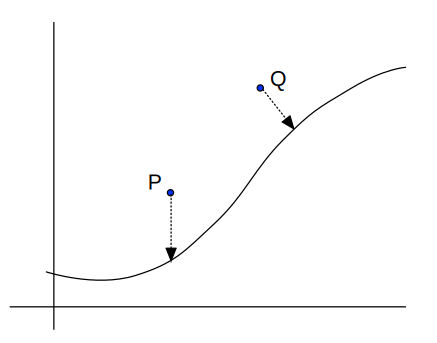
\includegraphics[width=0.5\textwidth,height=\textheight]{FilteringFigures/proj2model.*}
\caption{}
\end{figure}

Say that you have a data set: \((x_i, y_i),\quad  i=1, \dots, k.\) and
you want to fit a model to it (project onto a model):

\[y = a_n x^n + a_{n-1}x^{n-1} + \dots + a_1x + a_0 , \quad\quad  k >> n\]

or in general

\[y = a_n \phi_n(x) + a_{n-1}\phi_{n-1}(x) + \dots + a_0 \phi_0(x)\]

How does one use the data to find the coefficients of the model?

Plug the data into the model:

\[\begin{aligned}
\begin{array}{l}
y_1 = a_n x_1^n + a_{n-1}x_1^{n-1} + \dots + a_1x_1 + a_0 \\[3mm]
y_2 = a_n x_2^n + a_{n-1}x_2^{n-1} + \dots + a_1x_2 + a_0 \\[3mm]
\vdots \\[3mm]
y_{k-1} = a_n x_{k-1}^n + a_{n-1}x_{k-1}^{n-1} + \dots + a_{k-1}x_{k-1} + a_0 \\[3mm]
y_k = a_n x_k^n + a_{n-1}x_k^{n-1} + \dots + a_1x_k + a_0
\end{array}
\end{aligned}\]

This can be rewritten in the language of linear algebra:

Plug the data into the model:

\[\begin{aligned}
\underbrace{\begin{bmatrix} y_1 \\[3mm] y_2 \\[3mm] \vdots \\[3mm] y_k \end{bmatrix}}_y =
\underbrace{ \begin{bmatrix} x_1^n & x_1^{n-1} & \dots & x_1 & 1 \\[3mm]
x_2^n & x_2^{n-1} & \dots & x_2 & 1 \\[3mm]
\vdots &\vdots & & \vdots & \vdots\\[3mm]
x_k^n & x_k^{n-1} & \dots & x_k & 1
\end{bmatrix} }_X
\underbrace{\begin{bmatrix}
a_n \\[3mm] a_{n-1} \\[3mm] \vdots \\[3mm] a_1 \\[3mm] a_0
\end{bmatrix}}_a
\end{aligned}\]

The problem is that this system is not usually square and so one cannot
just invert the matrix \(X\) to find the coefficients \(a_j\).
Expressing our system as

\[y = X a\]

We assume that we have many data points but wish a low degree polynomial
to fit the data points, \(k >> n+1\) where \(k\) is the number of points
and \(n\) is the degree of the polynomial. This is an overdetermined
problem and presents us with a non-square matrix \(A\). We form the
normal equations

\[X^T y = X^TXa\]

we obtain a solvable system. If \(X^T X\) is of full rank, then we can
invert

\[a = \left(X^T X\right)^{-1} X^Ty\]

Once \(a\) is found then we may use

\[\hat{y} = a_n x^n + a_{n-1}x^{n-1} + \dots + a_1x + a_0\]

as the "fit" to the data.

Before we put this to use, we should address the question "is \(X^TX\)
of full rank?" What does this mean? Here it means that the columns must
be linearly independent. The geometric structure of the system looks
like:

\begin{figure}
\centering
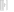
\includegraphics[width=0.3\textwidth,height=\textheight]{FilteringFigures/vrect.*}
\caption{}
\end{figure}

It is clear that if we have more rows than columns, the rows cannot be
linearly independent. The columns might be L.I.. If they are not then
two of the basis elements \(\phi_i(x)\) and \(\phi_j(x)\) are the same
and we have repeated one.

For this example, we have 20 points for which we would like to fit a
quadratic equation. Assume the data is contained in a file named
"data.txt" (with the same formatting), we can plot this using:

\(x_i\) \(y_i\)

\begin{verbatim}
0.026899  1.367895
0.115905  1.295606
0.250757  1.156797
0.413750  1.144025
0.609919  0.862480
0.669044  0.827181
0.868043  0.693536
1.080695  0.528216
1.233052  0.549789
1.312322  0.741778
1.402371  0.879171
1.724433  0.784356
1.844290  0.912907
1.901078  0.902587
2.117728  1.032718
2.235872  1.133116
2.331574  1.331071
2.607533  1.768845
2.719074  1.723766
2.853608  1.898702
\end{verbatim}

\begin{figure}
\centering
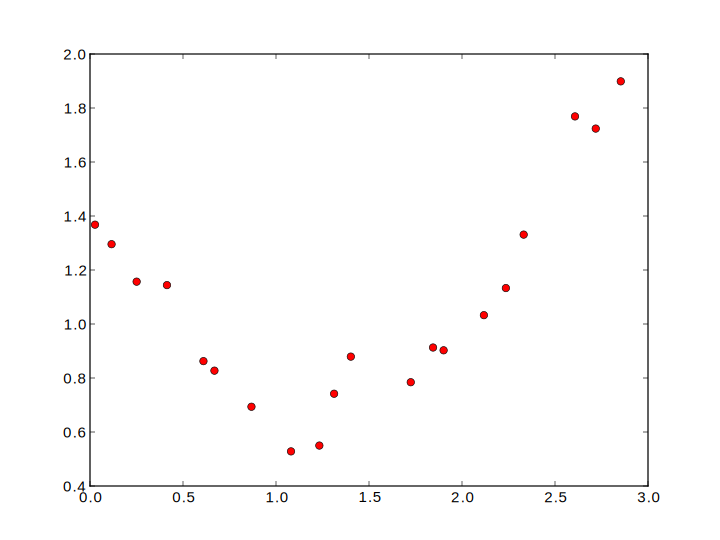
\includegraphics[width=0.85\textwidth,height=\textheight]{FilteringFigures/quadpts.*}
\caption{}
\end{figure}

Assume that the model for the data is \(y = a_2x^2 + a_1x +a_0\). Find
\(a_2, a_1, a_0\). Note that the system arises:

\begin{quote}
\[\begin{aligned}
\begin{array}{c}
   (0.026899, 1.367895) \to\quad 1.367895 = a_2(0.026899)^2 + a_1(0.026899) + a_0\\
   (0.115905,  1.295606) \to\quad  1.295606 = a_2(0.115905)^2 + a_1(0.115905) + a_0\\
    (0.250757, 1.156797) \to\quad   1.156797 = a_2(0.250757)^2 + a_1(0.250757) + a_0\\
   \vdots
  \end{array}
\end{aligned}\]
\end{quote}

which can be written as

\[\begin{aligned}
\begin{bmatrix}
(0.026899)^2 & 0.026899 & 1\\
(0.115905)^2 & 0.115905 & 1\\
(0.250757)^2 & 0.250757 & 1\\
\vdots & \vdots & \vdots
\end{bmatrix}
\begin{bmatrix}
 a_2 \\ a_1 \\ a_0
\end{bmatrix}
=
\begin{bmatrix}
 1.367895\\
  1.295606\\
 1.156797\\
\vdots
\end{bmatrix}
\end{aligned}\]

The Normal Equations can be formed

\[\begin{aligned}
\begin{bmatrix}
 (0.026899)^2 & (0.115905)^2 & (0.250757)^2 & \dots \\
 0.026899& 0.115905 & 0.250757 & \dots \\
1 & 1 & 1 & \dots
\end{bmatrix}
\begin{bmatrix}
(0.026899)^2 & 0.026899 & 1\\
(0.115905)^2 & 0.115905 & 1\\
(0.250757)^2 & 0.250757 & 1\\
\vdots & \vdots & \vdots
\end{bmatrix}
\begin{bmatrix}
 a_2 \\ a_1 \\ a_0
\end{bmatrix}
\end{aligned}\]

\[\begin{aligned}
=
\begin{bmatrix}
 (0.026899)^2 & (0.115905)^2 & (0.250757)^2 & \dots \\
 0.026899& 0.115905 & 0.250757 & \dots \\
1 & 1 & 1 & \dots
\end{bmatrix}
\begin{bmatrix}
 1.367895\\
  1.295606\\
 1.156797\\
\vdots
\end{bmatrix}
\end{aligned}\]

One can solve \(X^TX a = X^T y\): \(a = (X^TX)^{-1} X^T y\)

\begin{quote}
\[\begin{aligned}
\begin{bmatrix}
286.78135686  & 122.11468009 &  55.44347326 \\
 122.11468009 &  55.44347326  & 28.317947 \\
  55.44347326 &  28.317947  &   20.
\end{bmatrix}
\begin{bmatrix}
a_2 \\ a_1 \\ a_0
\end{bmatrix}
=
\begin{bmatrix}
  72.4241925 \\  33.380646 \\ 21.534542
\end{bmatrix}
\end{aligned}\]
\end{quote}

\[\begin{aligned}
\begin{bmatrix}
a_2 \\ a_1 \\ a_0
\end{bmatrix}
\approx
\begin{bmatrix}
 0.4930957 \\ -1.212858 \\ 1.42706\\
\end{bmatrix}
\end{aligned}\]

The curve is approximately \(y = 0.49x^2 - 1.21x + 1.42\), Figure~
\texttt{plot:quadgraph}

\begin{quote}
The plot of \(y = 0.49x^2 - 1.21x + 1.42\).
\end{quote}

\begin{Shaded}
\begin{Highlighting}[]
\KeywordTok{using}\NormalTok{ LinearAlgebra}

\NormalTok{N }\OperatorTok{=}\NormalTok{ length(xl)}
\NormalTok{x }\OperatorTok{=} \DataTypeTok{Float64}\NormalTok{[xl}\OperatorTok{;}\NormalTok{]}
\NormalTok{y }\OperatorTok{=} \DataTypeTok{Float64}\NormalTok{[yl}\OperatorTok{;}\NormalTok{]}
\NormalTok{xx }\OperatorTok{=}\NormalTok{ x}\OperatorTok{.*}\NormalTok{x}
\CommentTok{\# A is equivalent to AT in Python vice versa}
\NormalTok{A }\OperatorTok{=}\NormalTok{ transpose(}\DataTypeTok{Float64}\NormalTok{[xx x ones(N)])}
\NormalTok{AT }\OperatorTok{=} \DataTypeTok{Float64}\NormalTok{[xx x ones(N)]}
\NormalTok{AA }\OperatorTok{=}\NormalTok{ (A }\OperatorTok{*}\NormalTok{ AT)}
\NormalTok{ATy }\OperatorTok{=}\NormalTok{ (A }\OperatorTok{*}\NormalTok{ y)}

\NormalTok{c }\OperatorTok{=}\NormalTok{ (AA}\OperatorTok{\textbackslash{}}\NormalTok{ATy)}
\NormalTok{t }\OperatorTok{=} \DataTypeTok{Float64}\NormalTok{[}\FloatTok{0}\OperatorTok{:}\FloatTok{0.1}\OperatorTok{:}\FloatTok{2.9}\OperatorTok{;}\NormalTok{]}
\NormalTok{tt }\OperatorTok{=}\NormalTok{ t}\OperatorTok{.*}\NormalTok{t}
\CommentTok{\# This B is the same as the B transpose in python}
\NormalTok{B }\OperatorTok{=} \DataTypeTok{Float64}\NormalTok{[tt t ones(length(t))]}
\NormalTok{s }\OperatorTok{=}\NormalTok{ (B }\OperatorTok{*}\NormalTok{ c)}
\NormalTok{p }\OperatorTok{=}\NormalTok{ plot(t}\OperatorTok{,}\NormalTok{s)}
\NormalTok{plot}\OperatorTok{!}\NormalTok{(p}\OperatorTok{,}\NormalTok{x}\OperatorTok{,}\NormalTok{y}\OperatorTok{,}\NormalTok{ seriestype }\OperatorTok{=}\NormalTok{ scatter}\OperatorTok{,}\NormalTok{ xlims }\OperatorTok{=}\NormalTok{ (}\FloatTok{0}\OperatorTok{,}\FloatTok{3}\NormalTok{)}\OperatorTok{,}\NormalTok{ ylims }\OperatorTok{=}\NormalTok{ (}\FloatTok{0}\OperatorTok{,}\FloatTok{2}\NormalTok{) )}
\end{Highlighting}
\end{Shaded}

A couple of figures can help. For the following, we generate a segment
of a curve \(y=x^2-2x+1\) and add some noise. In
\texttt{plot:noisycurve1} the points with the added noise are show in
red and the least squares quadratic fit is shown in blue.

\begin{quote}
A data set with noise shown in red and the least squares fit is shown in
blue.
\end{quote}

Going a bit further, the noise is extracted and shown in yellow. The
blue curve is the least squares fit and the green curve is the original
polynomial.

\begin{quote}
The red curve is the sample or noisy set. The blue curve is the least
squares interpolant. Subtracting the interpolant from the original set
gives us the noise curve shown in yellow. The original data is shown in
green.
\end{quote}

\hypertarget{moore-penrose-pseudo-inverse}{%
\subsection{Moore-Penrose
Pseudo-Inverse}\label{moore-penrose-pseudo-inverse}}

Recall from linear algebra that we have two types of pseudo-inverses.
One that acts on the left one that acts on the right. They each address
complementary problems in least squares solutions to non-square systems.
These are reproduced here for convenience.

\begin{enumerate}
\item
  Left Moore-Penrose Pseudo-Inverse:
  \(H^+ = \left(H^TH\right)^{-1} H^T :\) \(H^+ H =I\)

  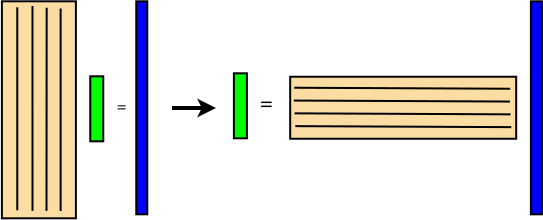
\includegraphics[width=0.75\textwidth,height=\textheight]{FilteringFigures/vrectsoln.*}
\item
  Right Moore-Penrose Pseudo-Inverse:
  \(H^+ = H^T \left(HH^T\right)^{-1}:\) \(H H^+ =I\)

  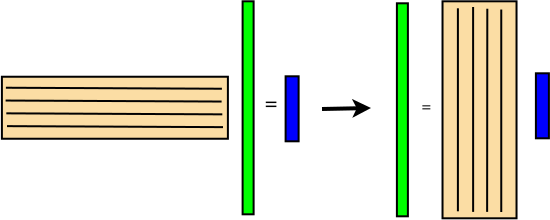
\includegraphics[width=0.75\textwidth,height=\textheight]{FilteringFigures/hrectsoln.*}
\end{enumerate}

\hypertarget{least-squares-observer}{%
\subsection{\texorpdfstring{\texttt{Least\ Squares\ Observer}}{Least Squares Observer}}\label{least-squares-observer}}

Least Squares is used because there is noise in the data collection or
the observations. Here we will summarize the material above and use a
notation closer to what is used in the Kalman Filter. Let's start with a
familiar example. Assume that you have a collection of similar sensors
(equal standard deviations for now) that you gather measurements from:
\(z_1\), \(z_2\), \ldots, \(z_n\). You know that they are noisy versions
of a hidden state \(x\), with noise \(w\) meaning that \(z = Hx + w\),
the observation of \(x\) subject to noise \(w\). Given \(k\)
observations \(z\) of state \(x\in{\Bbb R}^n\), \(k>>n\), with noise
\(w\):

\[z = Hx+w.\]

As before, we aim to find \(\hat{x}\) which minimizes the square error:

\[\| z - H\hat{x}\|.\]

So, we are seeking the least square solution to \(z = H\hat{x}\) which
is

\[\hat{x} = \left(H^TH\right)^{-1} H^T z.\]

The difference between the estimate and the actual value

\[\hat{x}-x = \left(H^TH\right)^{-1} H^T (Hx+w) -x
= \left(H^TH\right)^{-1} H^T w\]

If \(w\) has zero mean then \(\hat{x}-x\) has zero mean and \(\hat{x}\)
is an unbiased estimate (as we had before).

\hypertarget{example}{%
\subsubsection{Example}\label{example}}

In this example we observe just the state variable and without noise we
would just have \(z  = x\). Using this as our model we obtain a set of
equations:

\[\begin{aligned}
\begin{array}{c}
z_1 = x + w_1 \\
z_2 = x  + w_2\\
\vdots \\
z_n = x + w_n.\\
\end{array}
\end{aligned}\]

We have solved this problem earlier, but this time we will rewrite it in
a matrix form. Bear with me since it is a lot of machinery for a simple
problem, but it will help lead us to the more general case which
follows. It can be written as

\[z = Hx + w\]

where

\[\begin{aligned}
z = \begin{pmatrix} z_1 \\ z_2 \\ \vdots \\ z_n \end{pmatrix}, \quad  w = \begin{pmatrix} w_1 \\ w_2 \\ \vdots \\ w_n \end{pmatrix},\quad
H = \begin{bmatrix} 1 \\ 1 \\ \vdots \\ 1 \end{bmatrix}.
\end{aligned}\]

Write out the estimate to see how it compares to the previous one:

\[\begin{aligned}
\hat{x} = \left(H^TH\right)^{-1} H^T z = \left(\begin{bmatrix} 1 & 1 & \dots & 1\end{bmatrix} \begin{bmatrix} 1 \\ 1 \\ \vdots \\ 1 \end{bmatrix}\right)^{-1} \left( \begin{bmatrix} 1 & 1 & \dots & 1\end{bmatrix} \begin{pmatrix} z_1 \\ z_2 \\ \vdots \\ z_n \end{pmatrix}\right)
\end{aligned}\]

\[= \frac{1}{n} \sum_{i=1}^{n} z_i\]

which agrees with our earlier work (and below we will show that the
weighted one works out as well). The strength of this approach is in the
ease of generalization\footnote{Generalization is not our goal, we have
  a specific problem to address.}.

\hypertarget{weighted-least-squares-observer}{%
\subsubsection{Weighted Least Squares
Observer}\label{weighted-least-squares-observer}}

Traditional least squares is formulated by minimizing using the normal
innerproduct:

\[x^Ty = \sum_i x_iy_i.\]

If the inner product is weighted:

\[x^Ty = \sum_i x_i y_i q_i = x^T Q y\]

then the weighted least squares solution to

\[z = Hx + w\]\[is\]

\[\hat{x} = \left(H^T Q H\right)^{-1} H^TQz .\]

The matrix \(Q\) is any matrix for which the innerproduct above is a
valid. However, we will select \(Q\) as a diagonal matrix containing the
reciprocals of the variances (the reason shown below in the covariance
computation). We can rework our simple example:

\[\begin{aligned}
z = \begin{pmatrix} z_1 \\ z_2 \\ \vdots \\ z_n \end{pmatrix},  \quad w = \begin{pmatrix} w_1 \\ w_2 \\ \vdots \\ w_n \end{pmatrix}, \quad
H = \begin{bmatrix} 1 \\ 1 \\ \vdots \\ 1 \end{bmatrix}
\end{aligned}\]

and

\[\begin{aligned}
Q =
\begin{bmatrix}
\sigma_1^{-2} & 0 & \dots & 0 \\
0 & \sigma_2^{-2} &  \dots & 0  \\
0 & 0 &  \dots & 0  \\
0 & 0 & 0 &\sigma_n^{-2}  \\
\end{bmatrix}.
\end{aligned}\]

The estimate, \(\hat{x}\) is then
\(\hat{x} = \left(H^TQH\right)^{-1} H^T Q z\),

\[\begin{aligned}
\hat{x}= \left(\begin{bmatrix} 1 & 1 & \dots & 1\end{bmatrix}\begin{bmatrix}
\sigma_1^{-2} & 0 & \dots & 0 \\
0 & \sigma_2^{-2} &  \dots & 0  \\
0 & 0 &  \dots & 0  \\
0 & 0 & 0 &\sigma_n^{-2}  \\
\end{bmatrix} \begin{bmatrix} 1 \\ 1 \\ \vdots \\ 1 \end{bmatrix}\right)^{-1}
\end{aligned}\]

\[\begin{aligned}
\times \left( \begin{bmatrix} 1 & 1 & \dots & 1\end{bmatrix} \begin{bmatrix}
\sigma_1^{-2} & 0 & \dots & 0 \\
0 & \sigma_2^{-2} &  \dots & 0  \\
0 & 0 &  \dots & 0  \\
0 & 0 & 0 &\sigma_n^{-2}  \\
\end{bmatrix}\begin{pmatrix} z_1 \\ z_2 \\ \vdots \\ z_n \end{pmatrix}\right) ,
\end{aligned}\]

\[\hat{x}=\displaystyle \frac{\displaystyle \sum_{i=1}^n \frac{z_i}{\sigma_i^2}}
{\displaystyle \sum_{i=1}^n \frac{1}{\sigma_i^2}}\]

The covariance of this estimate is

\[= \left(H^TQH\right)^{-1} H^T Q\, W\, Q H\left(H^TQH\right)^{-1}\]

Often one selects the weighting to be inversely proportional to \(W\)
(the matrix of reciprocal variances) which is what we did above:

\[Q = W^{-1}.\]

A smaller standard deviation means better data, and thus we weigh this
more. Substituting in

\[\hat{x} = \left(H^T W^{-1} H\right)^{-1} H^TW^{-1}z\]

with covariance

\[P = \left(H^T W^{-1} H\right)^{-1}\]

Given an observation \(z\) of state \(x\) with noise \(w\):

\[z = Hx+w\]

the \(\hat{x}\) which minimizes the square error

\[\| z - H\hat{x}\|\]

\[\hat{x} = H^+z = W^{-1} H^T\left(H W^{-1} H^T\right)^{-1}z\]

with \(W\) the covariance of \(w\) and error covariance

\[P = \left(H W^{-1} H^T\right)^{-1}\]

if we take the same weighting as before.

\hypertarget{kalman-example-1}{%
\subsubsection{Example}\label{kalman-example-1}}

Assume that we have two state variables \(x_1\) and \(x_2\) and we are
able to observe the first directly (with noise) and the sum of the two
(with noise). The model will be two constants we are observing through a
noisy observation process. This means:

\[\begin{aligned}
z = Hx \quad \Rightarrow \quad
\begin{bmatrix}
 z_1 \\ z_2
\end{bmatrix}
=
\begin{bmatrix}
 1 & 0 \\
1 & 1
\end{bmatrix}
\begin{bmatrix}
 x_1 \\ x_2
\end{bmatrix}
+
\begin{bmatrix}
 w_1 \\ w_2
\end{bmatrix}
\end{aligned}\]

Multiple observations give:

\[\begin{aligned}
\begin{bmatrix}
 z_1 \\ z_2 \\ z_3 \\ z_4 \\ \vdots
\end{bmatrix}
=
\begin{bmatrix}
 1 & 0 \\
1 & 1  \\
1 & 0 \\
1 & 1  \\
\vdots & \vdots
\end{bmatrix}
\begin{bmatrix}
 x_1 \\ x_2
\end{bmatrix}
+
\begin{bmatrix}
 w_1 \\ w_2 \\ w_3 \\ w_4\\ \vdots
\end{bmatrix}
\end{aligned}\]

The least square solution to \(z = H\hat{x}\) is

\[\hat{x} = \left(H^TH\right)^{-1} H^T z\]

Assume we have data:

\begin{verbatim}
0.874328560532
3.25683958794
0.859486711669
2.86834487616
1.25271217589
2.95373764186
0.881013871661
3.09066238259
0.971121996741
3.03754386081
\end{verbatim}

Compute Normal Equation:

\[\begin{aligned}
H^T H =
\begin{bmatrix}
10 & 5 \\ 5 & 5
\end{bmatrix}
\quad \quad
H^Tz =
\begin{bmatrix}
 20.04579167  \\15.20712835
\end{bmatrix}
\end{aligned}\]

Solve \(H^T H x = H^Tz\): Then:
\(x_1 = 0.96773266, ~~ x_2=  2.07369301\)

Note that the actual values were \(x_1 = 1, x_2=  2\)

\hypertarget{example-2}{%
\subsubsection{Example}\label{example-2}}

Recall that there are two forms of the Least Squares Inverse (the
Pseudoinverse). The examples above used the left inverse. That applied
when we had more equations than unknowns (or variables), the problem was
overdetermined. There will be times for which the reverse is true; that
we will have more unknowns than equations. For the underdetermined
problem we use the right inverse. The following illustrates this idea.

Say that the system can observe two of three variables: \((u,v)\) from
\((u,v,\theta)\),

\[\begin{aligned}
z_k = Hx_k \quad \Rightarrow \quad \begin{bmatrix} \xi_k \\ \eta_k \end{bmatrix}
=
\begin{bmatrix}
 1 & 0 & 0 \\
0 & 1 & 0
\end{bmatrix}
\begin{bmatrix}
 u_k \\ v_k \\ \theta_k
\end{bmatrix}
\end{aligned}\]

For this problem we solve using the right inverse:

\[x_k = H^+ z_k .\]

The reason can be seen by looking at the object to be inverted in the
two pseudo-inverse formulas:

\[\begin{aligned}
H^TH = \begin{bmatrix}
 1 & 0 & 0 \\
0 & 1 & 0 \\
0 & 0 & 0
\end{bmatrix} ,
\quad
HH^T = \begin{bmatrix}
 1 & 0  \\
0 & 1
\end{bmatrix}.
\end{aligned}\]

The left matrix is not invertable. A right pseudo-inverse

\[\begin{aligned}
\begin{bmatrix}
 u_k \\ v_k \\ \theta_k
\end{bmatrix}
=
\begin{bmatrix}
 1 & 0  \\
0 & 1 \\
0 & 0
\end{bmatrix}
\left(
\begin{bmatrix}
 1 & 0  \\
0 & 1
\end{bmatrix}
\right)^{-1}
\begin{bmatrix} \xi_k \\ \eta_k \end{bmatrix}
=
\begin{bmatrix}
 1 & 0  \\
0 & 1 \\
0 & 0
\end{bmatrix}
\begin{bmatrix} \xi_k \\ \eta_k \end{bmatrix}
=
\begin{bmatrix} \xi_k \\ \eta_k \\ 0 \end{bmatrix}
\end{aligned}\]

Effectively we have produced a projection. This projection restricted
our variables to the relevant observational data. It can then be used in
sensor fusion applications.

\hypertarget{example-3}{%
\subsubsection{Example 3}\label{example-3}}

Assume that we have a noisy data set \((x_i, y_i)\) which we know lies
on a line:

\begin{verbatim}
[[  0.          -5.65520482]
 [  0.10204082   4.53774258]
 [  0.20408163   3.71191423]
 [  0.30612245   1.44760549]
 [  0.40816327   0.88024529]
 [  0.51020408   4.25592703]
 [  0.6122449    0.81475181]
 [  0.71428571   0.9275501 ]
 [  0.81632653   2.70301802]
 [  0.91836735   5.74002313]
 [  1.02040816   1.27503184]
 [  1.12244898   3.82976944]
 [  1.2244898    2.34108935]
 [  1.32653061   6.44934519]
 [  1.42857143   6.10025845]
 [  1.53061224   2.0450073 ]
 [  1.63265306   8.08201653]
 [  1.73469388   3.79104473]
 [  1.83673469   5.40629739]
 [  1.93877551   4.15556209]
 [  2.04081633   4.49578503]
 [  2.14285714   7.48854739]
 [  2.24489796   5.07750616]
 [  2.34693878   4.29701526]
 [  2.44897959   7.20452521]
 [  2.55102041   6.72492257]
 [  2.65306122   7.56408995]
 [  2.75510204   7.2419468 ]
 [  2.85714286   3.45946936]
 [  2.95918367   3.54635642]
 [  3.06122449   5.54792305]
 [  3.16326531   8.60804178]
 [  3.26530612   5.41562294]
 [  3.36734694  10.3737351 ]
 [  3.46938776   7.89065344]
 [  3.57142857   6.86298534]
 [  3.67346939   7.81332673]
 [  3.7755102    8.55556688]
 [  3.87755102   9.56774192]
 [  3.97959184   8.10000457]
 [  4.08163265   8.98656353]
 [  4.18367347   6.34429316]
 [  4.28571429   4.62596754]
 [  4.3877551    5.46160224]
 [  4.48979592  11.6944026 ]
 [  4.59183673   9.44392528]
 [  4.69387755   8.49333718]
 [  4.79591837  12.5121096 ]
 [  4.89795918   7.59781085]
 [  5.           9.60759719]]
\end{verbatim}

If we know the formula for the line we can project onto the line. For
this example, we will assume we don't have the formula and are
attempting to deduce the line. Meaning the model is that the data has a
linear relation, we just lack the parameters. {[}So we are doing a
parametric curve fit.{]} We use the same approach as with previous
datasets. The model is \(y = a_1x + a_0\). Application of the data set
and we have an overconstrained system of equations. Using the left
pseudoinverse as before we can determine \(a_1, a_0\). We may get
something like \(a_1=2.2231\), \(a_0 =  1.0124\), see
\texttt{fig:LSnoiseReduction} for data and plot. How would this be a
filter? You can project points onto the line via the line projection
formula found in calculus: \(a = a_1\), \(b = -1.0\), \(c = a_0\),

\[\begin{aligned}
\begin{matrix}
\displaystyle d = a^2+b^2\\[5pt]
\displaystyle px = \frac{b(bx - ay)-ac}{d} \\[5pt]
\displaystyle py = \frac{a(-bx+ay)-bc}{d}
\end{matrix}
\end{aligned}\]

The application of this as a filter is shown in
\texttt{fig:LSnoiseReductionO}.

\begin{quote}
Dataset and least square fit. The data is in red, the curve fit is the
solid blue line and the projection of the data is the blue dots.

Projecting data onto the line as a filter. Green dots are new data, the
curve fit is the solid blue line and blue dots are their projections.
\end{quote}

\textbf{Footnotes}
